\documentclass[a4paper]{exam}

\usepackage{geometry}
\usepackage{graphicx}
\usepackage{hyperref}
\usepackage{mathtools}
\usepackage{titling}

\printanswers

\title{Weekly Challenge 04: Sorting algorithms\\CS 412 Algorithms: Design and Analysis}
\author{q1-team-2}  % <==== replace with your team name for grading
\date{Habib University | Spring 2023}

\runningheader{CS 412: Algorithms}{WC04: Sorting algorithms}{\theauthor}
\runningheadrule
\runningfootrule
\runningfooter{}{Page \thepage\ of \numpages}{}

\qformat{{\large\bf \thequestion. \thequestiontitle}\hfill}
\boxedpoints

\begin{document}
\maketitle

\begin{questions}


	\titledquestion{Average number of comparisons}

	We talked in class about comparison-based sorting algorithms. (Here is a \href{https://www.youtube.com/watch?v=kPRA0W1kECg&t=344s}{nice visual depiction} of some sorting algorithms.) Here, we will compare the average number of comparisons performed by different sorting algorithm.
	For a given algorithm, we record the number of comparisons that the algorithm makes for a given input. We run the algorithm over different inputs and take the average of the number of comparisons over all the inputs.

	\subsection*{Tasks}
	\begin{description}
		\item[Implementation] Obtain or write implementations of at least 5 different comparison-based sorting algorithms, e.g., insertion, selection, bubble, quick, merge, shell, heap, and/or any others. Modify each implementation to obtain a count of the total number of comparisons performed for a given input.
		\item[Average comparisons] For a given $n$, generate $10\lceil \log_2 n \rceil$ random permutations of the set, $\{1,2,\ldots,n\}$. Obtain the average number of comparisons performed by each algorithm on this set of inputs.
		\item[Compare] Generate a plot of the average number of comparisons performed by each algorithm over a wide range of values of $n$, e.g. \texttt{n in range(1000,500001,1000)}. Include the plot below along with any observations or insights that you find worth mentioning.
		\item[Share] Share your plot as a comment on the \href{https://web.yammer.com/main/org/habib.edu.pk/threads/eyJfdHlwZSI6IlRocmVhZCIsImlkIjoiMjExNDMxMzQ1MDUwNDE5MiJ9}{WC04 post} in the course group.
		\item[Plot readability] Make sure that each plot is clearly labeled, or the diagram contains a clearly visible legend. Make sure that the axis limits are set such that the plots are clearly visible and occupy a large portion of the diagram. Include separate diagrams over different axis ranges if necessary.
		\item[Attribution] Adherence to the usual attribution practices is expected. Make sure to cite any external sources.
	\end{description}

	\begin{solution}
		% Enter your solution here.
		\\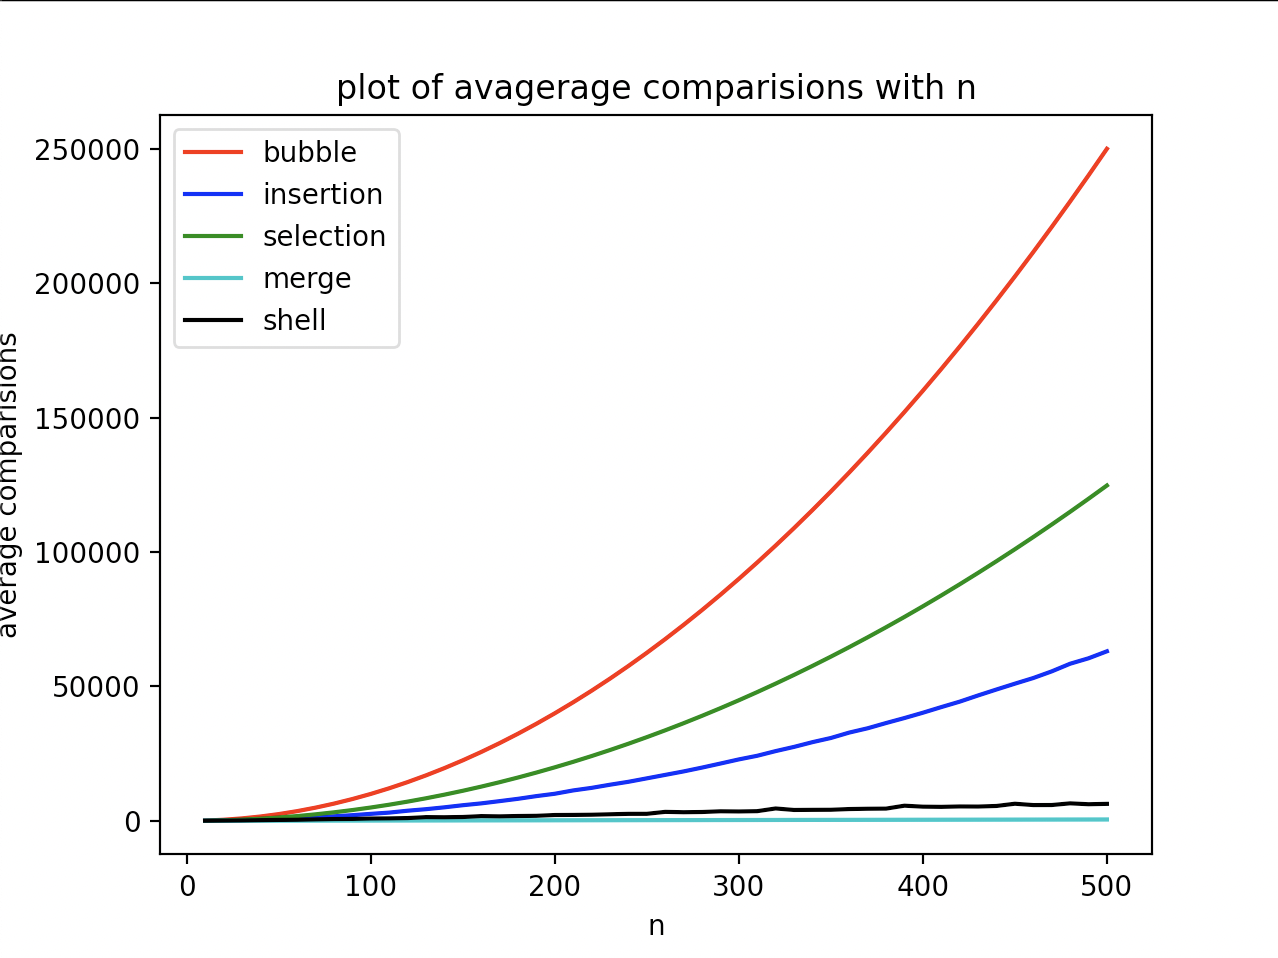
\includegraphics[scale =  0.5]{plot_(10,501,10).png}
		\\Bubble sort makes the most comparisons, it makes $n^2$ comparisons in every case. 
		Which makes the plot of $n$ to number of comparisions a quatradic function.
		\\Merge sort makes the least amout of comparisions. And the growth rate of the function is the slowest in merge sort and shell sort.
	\end{solution}

\end{questions}

\end{document}
